\documentclass[aspectratio=169]{beamer}

\usetheme{Boadilla}
\usefonttheme{professionalfonts}
\setbeamertemplate{navigation symbols}{}
\setbeamertemplate{itemize items}[circle]
\setbeamertemplate{enumerate items}[default]
\setbeamertemplate{headline}{}

\usepackage[utf8]{inputenc}
\usepackage[T1]{fontenc}
\usepackage{lmodern}
\usepackage{amsmath}
\usepackage{booktabs}
\usepackage{tabularx}
\usepackage{array}
\usepackage{hyperref}
\usepackage[strings]{underscore}
\usepackage{listings}
\usepackage{tikz}
\usetikzlibrary{arrows.meta,positioning,fit,calc,shapes.geometric}
\usepackage{xcolor}

\definecolor{courseblue}{HTML}{12355B}
\definecolor{coursegold}{HTML}{C98A2E}
\definecolor{courseice}{HTML}{EEF3F8}
\definecolor{coursegreen}{HTML}{2F6B4F}
\definecolor{coursegray}{HTML}{4B5563}
\definecolor{codebg}{HTML}{F7F9FC}
\definecolor{codecomment}{HTML}{5E6C84}
\definecolor{codestring}{HTML}{0B6E4F}

\setbeamercolor{palette primary}{bg=courseblue,fg=white}
\setbeamercolor{palette secondary}{bg=coursegold,fg=white}
\setbeamercolor{palette tertiary}{bg=courseblue,fg=white}
\setbeamercolor{palette quaternary}{bg=coursegold,fg=white}
\setbeamercolor{structure}{fg=courseblue}
\setbeamercolor{frametitle}{bg=courseice,fg=courseblue}
\setbeamercolor{title}{fg=courseblue}
\setbeamercolor{block title}{bg=courseblue,fg=white}
\setbeamercolor{block body}{bg=courseice,fg=black}
\setbeamercolor{normal text}{fg=black,bg=white}
\setbeamercolor{alerted text}{fg=coursegold}

\setbeamerfont{footline}{size=\scriptsize}

\setbeamertemplate{footline}{
  \leavevmode
  \hbox{
    \begin{beamercolorbox}[wd=.33\paperwidth,ht=2.8ex,dp=1.2ex,leftskip=0.8em]{palette primary}%
      University of Trieste
    \end{beamercolorbox}%
    \begin{beamercolorbox}[wd=.49\paperwidth,ht=2.8ex,dp=1.2ex,center]{palette tertiary}%
      \coursename{} \textbar{} \coursecode
    \end{beamercolorbox}%
    \begin{beamercolorbox}[wd=.18\paperwidth,ht=2.8ex,dp=1.2ex,rightskip=0.8em plus1fil]{palette secondary}%
      \insertframenumber{} / \inserttotalframenumber
    \end{beamercolorbox}%
  }
}

\hypersetup{
  colorlinks=true,
  linkcolor=courseblue,
  urlcolor=coursegreen
}

\lstdefinestyle{coursepython}{
  language=Python,
  basicstyle=\ttfamily\footnotesize,
  keywordstyle=\color{courseblue}\bfseries,
  commentstyle=\color{codecomment}\itshape,
  stringstyle=\color{codestring},
  showstringspaces=false,
  columns=fullflexible,
  keepspaces=true,
  frame=single,
  framerule=0.6pt,
  rulecolor=\color{courseblue},
  backgroundcolor=\color{codebg},
  xleftmargin=0.4em,
  xrightmargin=0.4em,
  aboveskip=0.4em,
  belowskip=0.2em
}

\newcommand{\coursename}{Data-driven Systems Engineering}
\newcommand{\coursecode}{440MI / 305SM}
\newcommand{\coursefooter}{}

\newcommand{\learninggoals}[1]{
  \begin{block}{Learning goals}
  #1
  \end{block}
}

\newcommand{\repoactivity}[1]{
  \begin{block}{Repo activity}
  #1
  \end{block}
}

\newcommand{\readinglist}[1]{
  \begin{block}{Papers and materials}
  {\footnotesize #1}
  \end{block}
}

\newcommand{\coursecontextframe}[5]{
  \begin{frame}{Course Map and Running Cases}
  \centering
  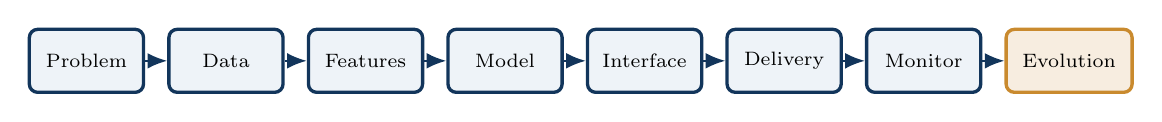
\begin{tikzpicture}[node distance=0.28cm]
  \node[flowbox, minimum width=1.45cm, minimum height=0.8cm] (problem) {\scriptsize Problem};
  \node[flowbox, minimum width=1.45cm, minimum height=0.8cm, right=of problem] (data) {\scriptsize Data};
  \node[flowbox, minimum width=1.45cm, minimum height=0.8cm, right=of data] (features) {\scriptsize Features};
  \node[flowbox, minimum width=1.45cm, minimum height=0.8cm, right=of features] (model) {\scriptsize Model};
  \node[flowbox, minimum width=1.45cm, minimum height=0.8cm, right=of model] (interface) {\scriptsize Interface};
  \node[flowbox, minimum width=1.45cm, minimum height=0.8cm, right=of interface] (delivery) {\scriptsize Delivery};
  \node[flowbox, minimum width=1.45cm, minimum height=0.8cm, right=of delivery] (monitor) {\scriptsize Monitor};
  \node[accentbox, minimum width=1.6cm, minimum height=0.8cm, right=of monitor] (evolution) {\scriptsize Evolution};
  \foreach \a/\b in {problem/data,data/features,features/model,model/interface,interface/delivery,delivery/monitor,monitor/evolution} {
    \draw[arrow] (\a) -- (\b);
  }
  \end{tikzpicture}

  \vspace{0.5em}
  \begin{block}{Today in the course}
  \textbf{Focus:} #1

  \textbf{Bridge:} #2
  \end{block}

  \begin{columns}[T]
  \column{0.48\textwidth}
  \begin{block}{Fraud case}
  {\footnotesize #3}
  \end{block}
  \column{0.48\textwidth}
  \begin{block}{Pasteurization case}
  {\footnotesize #4}
  \end{block}
  \end{columns}

  \vspace{0.3em}
  {\footnotesize \textbf{Course thread:} #5}
  \coursefooter
  \end{frame}
}

\newcommand{\classclosingframe}[4]{
  \begin{frame}{From This Class to the Next}
  \begin{block}{What stays with us}
  #1
  \end{block}

  \begin{columns}[T]
  \column{0.48\textwidth}
  \begin{block}{Project use}
  {\footnotesize #2}
  \end{block}
  \column{0.48\textwidth}
  \begin{block}{Next connection}
  {\footnotesize #3}
  \end{block}
  \end{columns}

  \vspace{0.3em}
  {\footnotesize \textbf{Course thread:} #4}
  \coursefooter
  \end{frame}
}

\tikzset{
  flowbox/.style={
    rounded corners=3pt,
    draw=courseblue,
    fill=courseice,
    very thick,
    minimum width=2.2cm,
    minimum height=0.9cm,
    align=center,
    font=\small
  },
  accentbox/.style={
    rounded corners=3pt,
    draw=coursegold,
    fill=coursegold!15,
    very thick,
    minimum width=2.2cm,
    minimum height=0.9cm,
    align=center,
    font=\small
  },
  arrow/.style={
    -{Latex[length=2.5mm,width=2mm]},
    thick,
    draw=courseblue
  }
}


\title{Class 14: Project Proposal and Delivery Planning}
\author{\coursename}
\date{}

\begin{document}

\frame{\titlepage \coursefooter}

\begin{frame}{Agenda}
\begin{itemize}
\item Why planning matters in ML projects
\item Project summary and scope
\item Deliverables and milestones
\item Work Breakdown Structure and sprint or Gantt planning
\item Definition of Ready and Definition of Done
\item Risks and governance for ML projects
\end{itemize}
\coursefooter
\end{frame}

\begin{frame}{Planning is part of the engineering work}
\learninggoals{
\begin{itemize}
\item Turn a project idea into scope, milestones, and deliverables.
\item Define what will be built first and what can wait.
\item Make project status visible through artifacts, not only verbal updates.
\item Connect proposal quality to later testing, deployment, and monitoring work.
\end{itemize}
}
\coursefooter
\end{frame}

\coursecontextframe
{Project planning as lifecycle design.}
{This class turns the course concepts into an executable project plan with milestones, deliverables, and evidence of progress.}
{In the fraud case, planning means sequencing data work, baseline modeling, service exposure, deployment checks, and monitoring criteria.}
{In the pasteurization case, planning means sequencing sensor understanding, forecasting or alerting logic, dashboard integration, and drift response design.}
{The course thread is that a coherent project proposal should already reflect the full lifecycle, not only the modeling step.}

\begin{frame}{Why planning matters in ML projects}
\begin{itemize}
\item ML systems evolve through data, code, models, interfaces, validation, and operations.
\item More roles means more handoffs, which means more need for shared artifacts.
\item A weak proposal creates downstream confusion in requirements, evaluation, and release planning.
\end{itemize}
\begin{block}{Practical claim}
Planning does not remove uncertainty, but it makes uncertainty visible enough to manage.
\end{block}
\coursefooter
\end{frame}

\begin{frame}{A project summary defines boundaries}
\begin{itemize}
\item What problem is being solved?
\item Who uses or is affected by the result?
\item What is in scope for this project?
\item What is intentionally out of scope?
\item What evidence will convince stakeholders that the project is useful?
\end{itemize}
\coursefooter
\end{frame}

\begin{frame}{What a strong project summary should contain}
\begin{itemize}
\item Problem statement and target users.
\item Data sources and expected constraints.
\item Expected system output: prediction, forecast, alert, or recommendation.
\item Success criteria tied to technical and user outcomes.
\item Risks, assumptions, and dependencies.
\end{itemize}
\coursefooter
\end{frame}

\begin{frame}{Objectives should be specific enough to evaluate}
\begin{block}{Weak objective}
Build an ML system for quality control.
\end{block}
\begin{block}{Stronger objective}
Detect abnormal process trajectories from synthetic pasteurization sensor data and expose alerts through a dashboard with traceable event logs.
\end{block}
\begin{itemize}
\item Strong objectives are specific, measurable, relevant, and bounded enough to review.
\end{itemize}
\coursefooter
\end{frame}

\begin{frame}{Milestones and WBS}
\begin{itemize}
\item Proposal approval
\item Data pipeline MVP
\item Baseline model
\item Deployable service or dashboard
\item Monitoring active
\item Final demonstration
\end{itemize}
\begin{block}{WBS reminder}
Break work into outputs that can be reviewed, not vague activity labels.
\end{block}
\coursefooter
\end{frame}

\begin{frame}{The WBS is about outputs, not vague activity}
\begin{itemize}
\item Good work packages end in something reviewable: cleaned dataset, baseline notebook, API endpoint, dashboard page, monitoring report.
\item The 100\% rule helps ensure the WBS covers the whole scope without duplication.
\item If a task cannot be evaluated by an external reviewer, it is often too vague.
\end{itemize}
\coursefooter
\end{frame}

\begin{frame}{Suggested semester deliverables}
\begin{enumerate}
\item Data understanding and requirement brief.
\item Baseline model and evaluation report.
\item Packaged service or dashboard.
\item CI/CD or reproducibility automation.
\item Monitoring or drift analysis plan.
\end{enumerate}
\coursefooter
\end{frame}

\begin{frame}{Deliverables should map to the lifecycle}
\begin{tabularx}{\textwidth}{>{\bfseries}l X}
Deliverable & Why it matters \\
\toprule
Data pipeline artifact & Makes inputs reproducible and inspectable. \\
Baseline model & Creates a reference point for later improvement. \\
Deployable interface & Proves the model can be consumed by users or systems. \\
Automation artifact & Reduces manual, unrepeatable work. \\
Monitoring plan & Shows how the system remains trustworthy after release. \\
\bottomrule
\end{tabularx}
\coursefooter
\end{frame}

\begin{frame}{Sprint and timeline thinking}
\begin{itemize}
\item Sprint 0: environment, repo structure, and scope.
\item Sprint 1: data understanding and requirements.
\item Sprint 2: baseline modeling.
\item Sprint 3: serving and integration.
\item Sprint 4: monitoring and final hardening.
\end{itemize}
\coursefooter
\end{frame}

\begin{frame}{Milestones reduce risk when they represent decisions}
\begin{itemize}
\item Proposal approval means the team has a coherent scope.
\item Data pipeline MVP means later modeling is grounded in real inputs.
\item Baseline model means performance can be compared instead of guessed.
\item Deployable service means integration risk is no longer abstract.
\item Monitoring active means the project is thinking beyond the demo.
\end{itemize}
\coursefooter
\end{frame}

\begin{frame}{A more suitable proposal example}
\begin{block}{Project}
Forecast temperature and detect abnormal state transitions in a synthetic pasteurization line.
\end{block}
\begin{itemize}
\item Data source: Flask stream from `pasteurization/serving.py`.
\item MVP: predict next temperature value and visualize drift alerts.
\item Stretch goal: state-aware forecasting and alert triage.
\item Main risks: synthetic realism, label scarcity, and operator-facing thresholds.
\end{itemize}
\coursefooter
\end{frame}

\begin{frame}{Another project pattern students can defend}
\begin{block}{Project}
Fraud scoring as a service for transaction review support.
\end{block}
\begin{itemize}
\item Data source: credit-card fraud dataset and engineered features.
\item MVP: classify transactions and expose a scoring endpoint.
\item Stretch goal: threshold tuning plus analyst-facing dashboard.
\item Risks: class imbalance, false-positive cost, and drift after deployment.
\end{itemize}
\coursefooter
\end{frame}

\begin{frame}{DoR and DoD for student teams}
\begin{columns}[T]
\column{0.48\textwidth}
\textbf{Definition of Ready}
\begin{itemize}
\item Requirement is written
\item Data source identified
\item Acceptance criteria drafted
\end{itemize}
\column{0.48\textwidth}
\textbf{Definition of Done}
\begin{itemize}
\item Code runs reproducibly
\item Result is documented
\item Test or demo evidence exists
\end{itemize}
\end{columns}
\coursefooter
\end{frame}

\begin{frame}{A lightweight risk register helps project control}
\begin{tabularx}{\textwidth}{>{\bfseries}l X}
Risk & Example response \\
\toprule
Data access or quality risk & Define fallback datasets and validation checks. \\
Model performance risk & Commit to a baseline and threshold review. \\
Integration risk & Deliver an API or dashboard slice early. \\
Schedule risk & Separate must-have deliverables from stretch goals. \\
Governance risk & Document assumptions, versions, and monitoring triggers. \\
\bottomrule
\end{tabularx}
\coursefooter
\end{frame}

\begin{frame}{What a strong proposal presentation should show}
\begin{itemize}
\item The problem and why it matters.
\item The system boundary and main users.
\item The data source, constraints, and risks.
\item The milestone sequence and what each one proves.
\item The evidence that the project is becoming an engineered system, not only a notebook.
\end{itemize}
\coursefooter
\end{frame}

\classclosingframe
{\begin{itemize}
\item A strong proposal defines the problem, the system boundary, the evidence plan, and the main risks.
\item Milestones should demonstrate engineering progress, not only analytical activity.
\item Good project planning anticipates delivery, monitoring, and change from the start.
\end{itemize}}
{This helps student teams present a believable path from data and baseline models to interfaces, deployment, and operational follow-up.}
{Class 15 closes the sequence with monitoring and drift response, showing how project plans must extend beyond first deployment.}
{Project planning becomes complete only when it includes how the system will be observed, corrected, and improved after release.}

\begin{frame}{Papers and materials}
\readinglist{
\href{https://proceedings.neurips.cc/paper_files/paper/2015/file/86df7dcfd896fcaf2674f757a2463eba-Paper.pdf}{Sculley et al. (2015), Hidden Technical Debt};\ 
\href{https://www.oreilly.com/library/view/designing-machine-learning/9781098107956/}{Designing Machine Learning Systems};\ 
\href{https://www.atlassian.com/agile/project-management/epics-stories-themes}{Project planning with epics and stories};\ 
\href{https://www.productplan.com/glossary/minimum-viable-product/}{Minimum Viable Product guide};\ 
\href{https://www.smartsheet.com/critical-path-method}{Critical path and schedule planning basics}.
}
\coursefooter
\end{frame}

\end{document}
